\chapter{Methods}\label{Methods}
The Methods chapter starts with an overview of the dataset selected for the fluid segmentation and intermediate slice synthesis tasks, while regarding the requirements needed for the training of each model and the reasoning behind the selection. Afterwards, it provides an explanation of the experiments that were performed during the dissertation, regarding fluid segmentation, inter-slice generation, and fluid volume estimation, while explaining the methodologies that were implemented.

\section{Dataset}
The application of deep learning to fluid segmentation in OCT volumes requires a large number of images annotated with the three retinal fluids for the training process. The manual segmentation of large amounts of B-scans is a laborious process, which results in a shortage of publicly available annotated OCT datasets. Consequently, the majority of these datasets contain a limited quantity of images.
\par
The dataset selected for this dissertation is the RETOUCH dataset \parencite{Bogunovic2019b}. This dataset consists of 112 OCT volumes, obtained with four different devices: 38 from the Cirrus HD-OCT (Zeiss Meditec), 38 from the Spectralis (Heidelberg Engineering), and 36 from the \mbox{T-1000}/T-2000 (Topcon). The 112 volumes are split into training (70 volumes) and testing (42 volumes). Only those in the training set have annotations of the retinal fluids (IRF, SRF, and PED). For the training and testing of the segmentation models, only the annotated volumes were used.
\par
From the 70 volumes, 24 were obtained with the Cirrus, 24 volumes were acquired with the Spectralis, and 22 were obtained with the two Topcon devices. The number of B-scans per volume, the dimensions of the B-scans, and the axial resolutions vary according to the device utilized to obtain the OCT. The volumes acquired using the Cirrus have 128 B-scans, while those obtained with Spectralis have 49 B-scans. The volumes acquired using Topcon devices (\mbox{T-1000} or \mbox{T-2000}) have 128 B-scans, but there are two volumes that only contain 64 \mbox{B-scans}. In total, 6838 B-scans were used on the train and test of the segmentation models.
\par
When compared with other renown OCT datasets annotated with retinal fluid, such as the Duke dataset \parencite{Chiu2015}, the two datasets from the University of Minnesota \parencite{Rashno2017, Rashno2018}, and the \textcite{Lu2019} dataset, the RETOUCH presents a significantly larger quantity of annotated volumes. It also shows more variety since the volumes were obtained using four different devices instead of including volumes from just one device, as done in the mentioned datasets. In Table \ref{tab:DatasetsSummary}, a comparison between the number of annotated B-scans in each of the mentioned datasets is shown, as well as the devices utilized to obtain the OCT images, the diseases of the patients, and the distribution of annotated B-scans per OCT volume.

\begin{table*}[!ht]
	\caption{Volumes, B-scans per volume, the total number of B-scans, and macular diseases in each dataset.}
	\centering
	\resizebox{\textwidth}{!}{\begin{tabular}{|c|c|c|c|c|c|}
		\hline
		& & & & & \\ [-1.5ex] % Used to center the text vertically
		& \textbf{DUKE2015 \cite{Chiu2015}} & \textbf{UMN2017 \cite{Rashno2017}} & \textbf{UMN2018 \cite{Rashno2018}} & \textbf{LU2019 \cite{Lu2019}} & \textbf{RETOUCH \cite{Bogunovic2019b}} \\ [1ex]
		\hline
		& & & & & \\ [-2.0ex]
		\textbf{Volumes} & 10 & 24 & 29 & 528 & 70$^{a}$ \\
		& & & & & \\ [-2.5ex]
		\textbf{B-scans/Volume} & 11 & 25 & 25 & Variable & 128 (Cirrus and Topcon$^{b}$), 64 (Topcon$^{b}$), 49 (Spectralis) \\
		& & & & & \\ [-2.5ex]
		\textbf{B-scans} & 110 & 600 & 725 & 750 & 6838 \\
		& & & & & \\ [-2.5ex]
		\textbf{Device} & Spectralis & Spectralis & Spectralis & Spectralis & Cirrus, Topcon and Spectralis \\
		& & & & & \\ [-2.5ex]
		\textbf{Disease} & DME & AMD & DME & DME & AMD and RVO \\
		\hline
		\multicolumn{4}{l}{}
	\end{tabular}}
	\label{tab:DatasetsSummary}
	\par
	\justifying
	\footnotesize{$^{a}$ 24 volumes from Cirrus, 22 volumes from Topcon, and 24 volumes from Spectralis.}
	\par 
	\justifying
	\footnotesize{$^{b}$ Two of the training volumes obtained using the Topcon devices have only 64 slices.}
\end{table*}

\par
For these reasons, the RETOUCH dataset is regarded as a diverse and large dataset, widely used in the literature that aims to perform fluid segmentation using deep learning, as done in \parencite{Rahil2023, Zhang2023, Xing2022, Tang2022, Liu2024, Li2023, Hassan2021b, Lu2019}. These aspects motivated the selection of the RETOUCH as the dataset that was used for implementing the models for fluid segmentation in OCT volumes in this dissertation.
\par
The best performing segmentation models were also evaluated on a private dataset provided by Centro Hospitalar Universitário de São João (CHUSJ). This dataset comprises six Spectralis OCT volumes, containing 19 slices each. The volumes vary in resolution, dimensions, noise levels, and contrasts, offering diverse testing scenarios. All volumes include at least one type of fluid, though the overall fluid presence is limited.
\par
Despite the scans in this dataset also being obtained with the Spectralis device, the resulting images had different shapes. In RETOUCH, all the Spectralis scans were of shape 496 $\times$ 512, while in CHUSJ dataset the images differ in width, depending on the OCT volume, with each B-scan's shape varying between 496 $\times$ 1024, 496 $\times$ 768, and 496 $\times$ 512. Since the images in this dataset did not contain the metadata informing the resolution of each slice, the slices had to be observed individually in order to determine whether the pixels in each B-scan corresponded to the same dimensions. In Figure \ref{fig:CHUSJDifferentResolutions}, slices with three different shapes are shown, where the differing resolutions from each image are visible.

\begin{figure}[!ht]
	\centering
	\includegraphics[width=1.0\linewidth]{figures/CHUSJDifferentResolutions.png}
	\caption{Three different B-scans with different dimensions (496 $\times$ 1024, 496 $\times$ 768, and 496 $\times$ 512, respectively) from the CHUSJ dataset. As shown in the scale at the bottom left of each B-scan, the resolutions are also differ depending on the slice.}
	\label{fig:CHUSJDifferentResolutions}
\end{figure}

In the same Figure, it also possible to see different image's characteristics. For example, in the left image, the choroid is very defined, while in the middle image it looks more blurry. The noise levels also differ depending on the image. The background in the left image shows almost no noise and the retinal layers are easily identifiable. In the middle image, some noise appears in the background and the retinal layers become harder to differentiate. Lastly, the image on the right contains noticeable background noise, while the retinal layers appear brighter than in the other images. 
\par
In the RETOUCH dataset, the volumes were extracted with consistent dimensions and noise levels across the same vendor. This results in visually similar images, whose differences can be attributed to the patient's characteristics. Therefore, while the differences seen in the CHUSJ dataset are a good test to understand the models' robustness, those trained in RETOUCH may not generalize well in this new dataset, as the visually similar images seen in training do not prepare the model for images with different visual appearances. In Figure \ref{fig:CHUSJProblematicImages}, three B-scans with really different characteristics are shown. The left B-scan is well oriented, but the choroid region is very defined, as opposed to the RETOUCH images where this region is blurry. The middle and right B-scan present an odd orientation and are much noisier than the examples seen in training.

\begin{figure}[!ht]
	\centering
	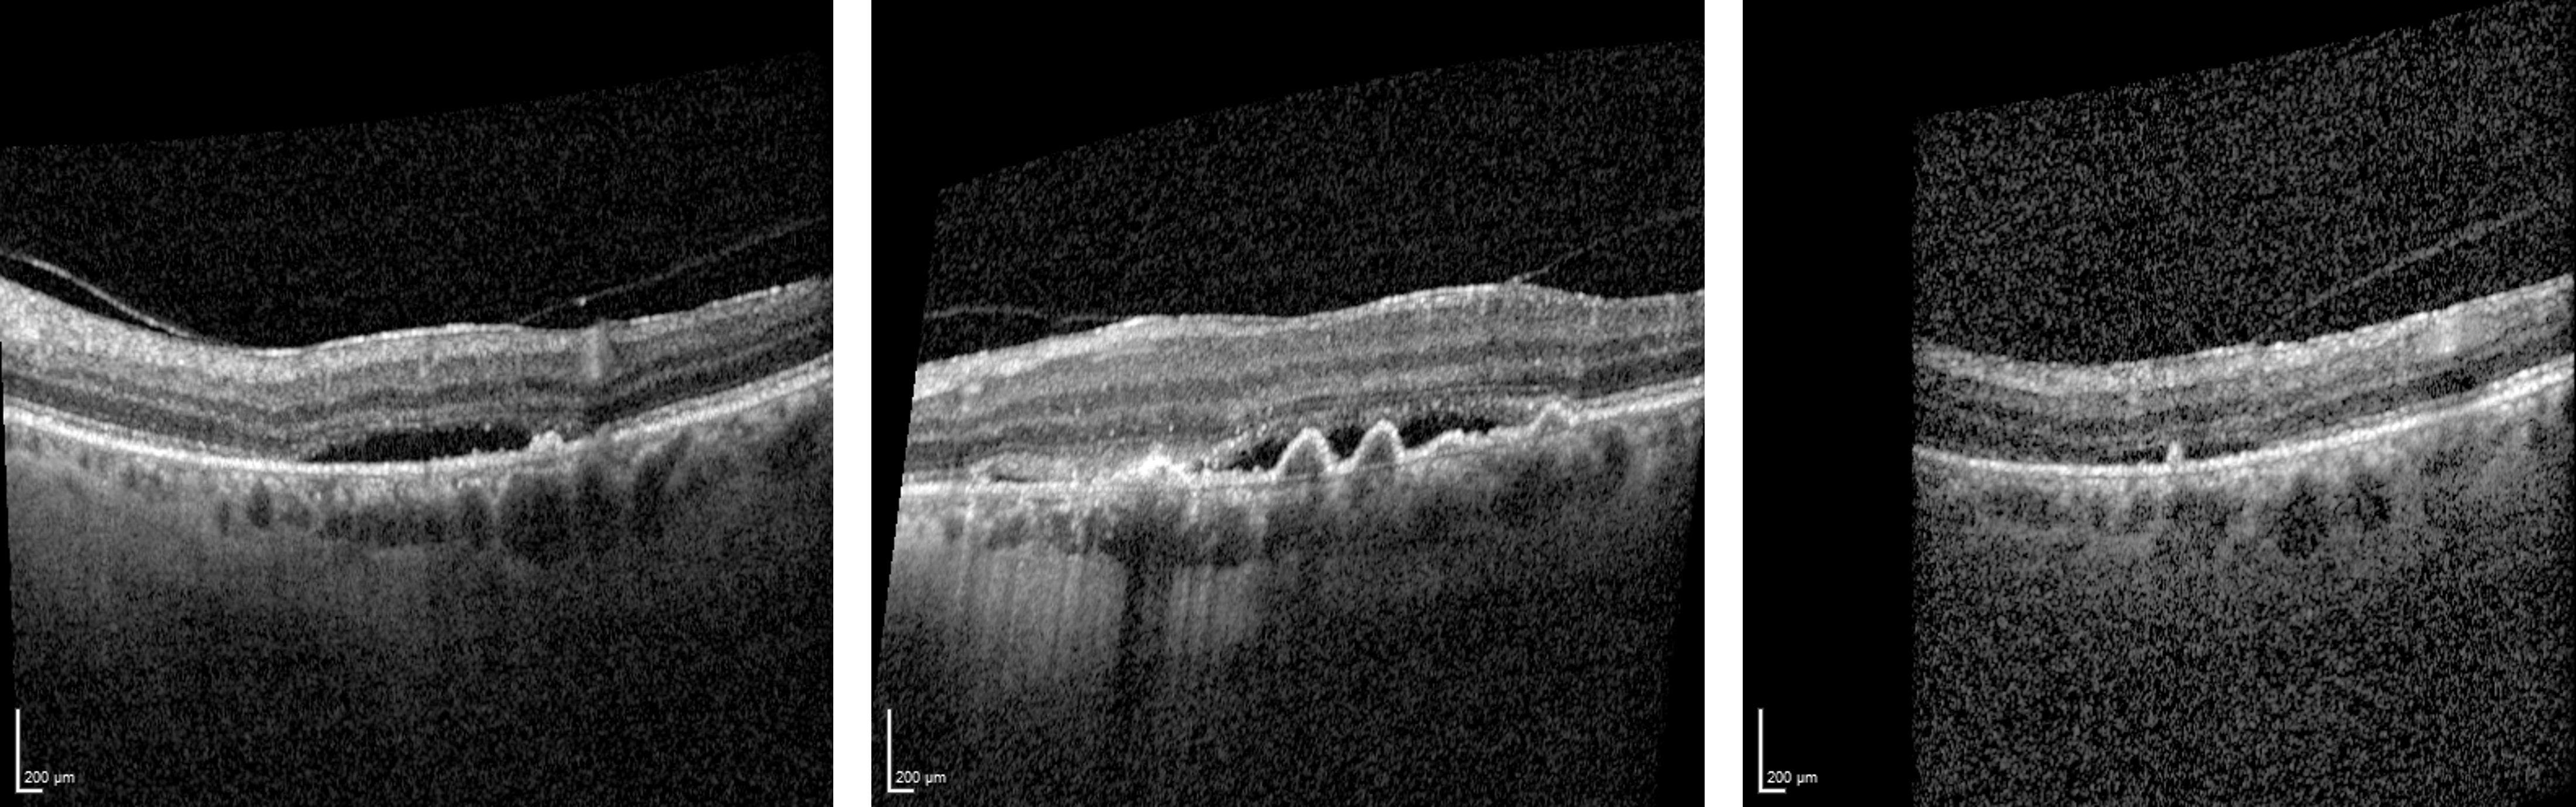
\includegraphics[width=1.0\linewidth]{figures/CHUSJProblematicImages.png}
	\caption{Three B-scans with characteristics different from those in RETOUCH. The left scan shows definition on the choroid, while the middle and right scan present an odd orientation and significant noise.}
	\label{fig:CHUSJProblematicImages}
\end{figure}

The last problem when considering segmentation masks from different sources is the criteria used in the segmentation. In medical images, the segmentation performed by different professionals may result in different outcomes, as shown in Figure \ref{fig:RETOUCHSegmentationDifferences}. Therefore, the criteria followed to segment fluid by the evaluator on CHUSJ dataset may be different from the criteria followed in the RETOUCH dataset. Furthermore, considering that in RETOUCH the approach to merge predictions by different evaluators is to consider both correct, the models trained in this data are prone to oversegment in unseen volumes.
\par
An example of different segmentation criteria between the RETOUCH and CHUSJ datasets is seen in Figure \ref{fig:RETOUCHvsCHUSJSegmentationCriteria}, where visually and anatomically similar regions are segmented only in one dataset. While in manual segmentation the context from the surrounding slices is relevant, the visual similarity between regions is the most important characteristic in the segmentation using CNNs. Therefore, when visually similar regions are not segmented equally or following the same criteria in the training and testing data, the predicted segmentation masks for the testing volumes may not coincide with the GT.

\begin{figure}[!ht]
	\centering
	\includegraphics[width=1.0\linewidth]{figures/RETOUCHSegmentationDifferences.png}
	\caption{Significantly different segmentations (middle images) of the same B-scan (left image) by different evaluators, in the RETOUCH dataset. The mask seen in cyan in the last image represents the final fluid regions when considering both evaluations \parencite{Bogunovic2019b}.}
	\label{fig:RETOUCHSegmentationDifferences}
\end{figure}

\begin{figure}[!ht]
	\centering
	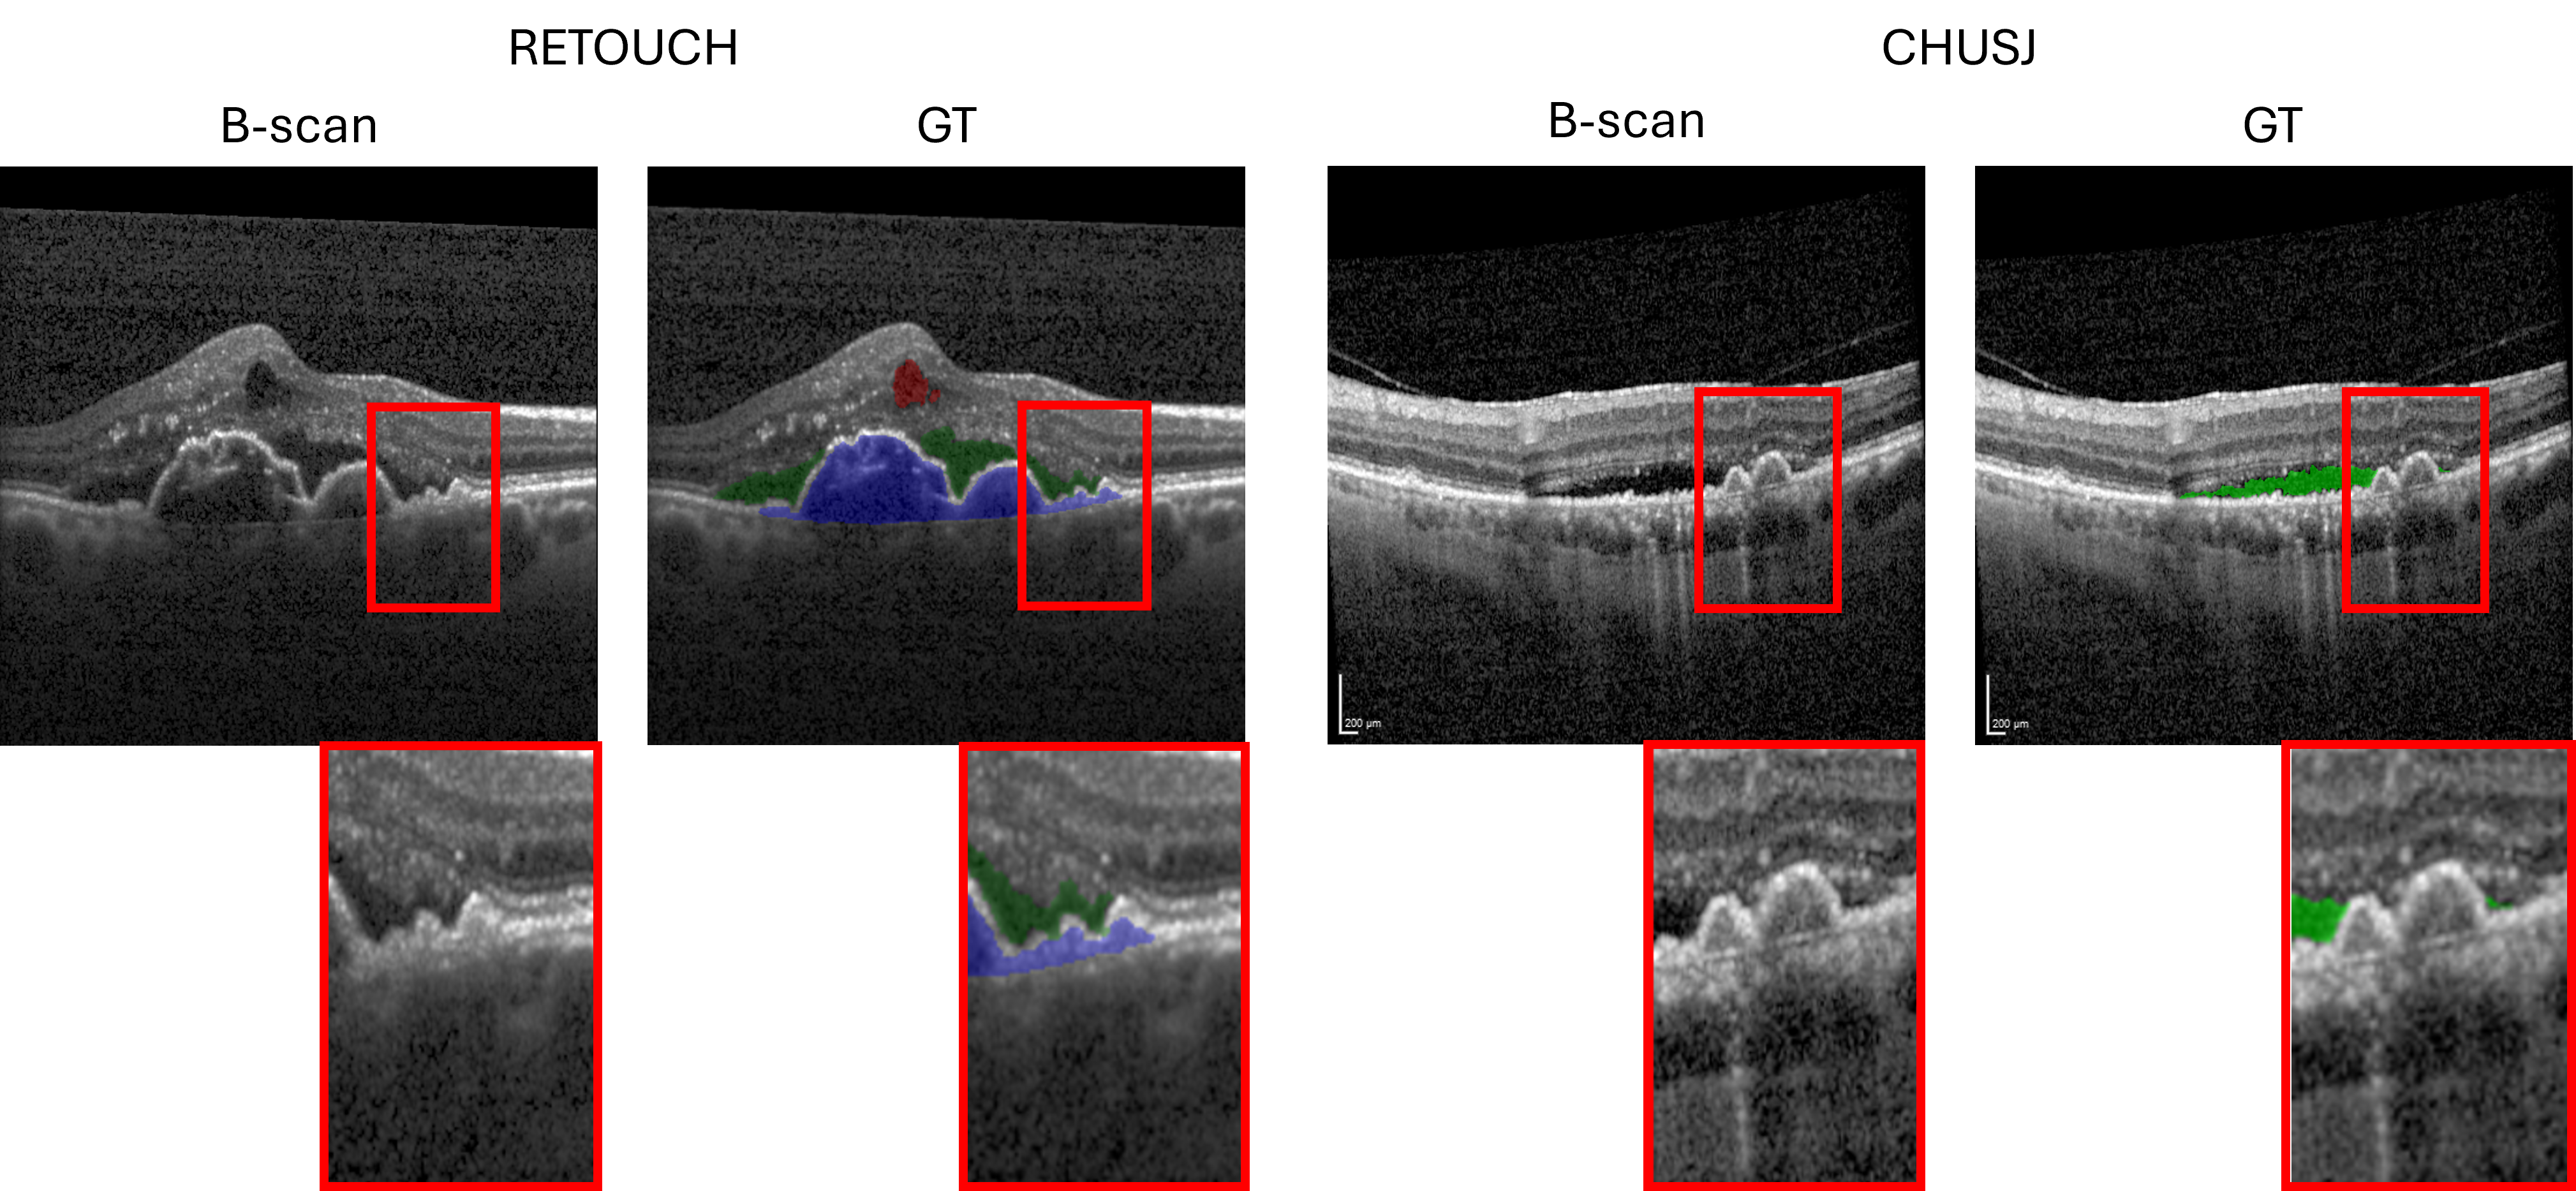
\includegraphics[width=1.0\linewidth]{figures/RETOUCHvsCHUSJSegmentationCriteria.png}
	\caption{Visually similar PED regions are segmented in one dataset but not on the other. This ambiguous segmentation can translate to worse performances in the model testing.}
	\label{fig:RETOUCHvsCHUSJSegmentationCriteria}
\end{figure}

\par
In intermediate slice synthesis, the 112 OCT volumes that constitute the RETOUCH dataset were used for the training and evaluation of the models. The volumes that do not have segmentation masks can also be included since these masks are not necessary in the intermediate slice generation task.
\par
The consistent number of slices per volume and large quantity of OCT volumes make the RETOUCH dataset suitable for the training and evaluation of the models developed to generate intermediate slices.

\section{Experiments}\label{Experiments}
In this subsection, the experiments conducted during the dissertation are explained in depth. The subsection begins with a description of how the data was split, followed by the experiments in fluid segmentation, intermediate slice generation, and in fluid volume estimation.
\par
All the experiments were conducted using an NVIDIA GeForce RTX 3080 GPU and the \hbox{PyTorch} machine learning library (version 2.5.1).

\subsection{Cross-validation}\label{CrossValidation}
To promote consistency across all experiments, the conditions were held identical. In every experiment, the train-test split followed a 5-fold split, with different splits being used for the segmentation and generation tasks. During training, all the images in three folds were utilized to train the model, while the images from one fold were used in its validation. One fold was reserved and used to compare the performance between the best model from different experiments. Therefore, four training runs are completed in each experiment, rotating the validation fold across runs. The reserved fold consists of the same OCT volumes for all experiments, allowing for further comparisons on data not seen by any of the models.
\par
The images in the fold that was used in validation allowed an insight of how the model was learning. In the segmentation experiments, the instance of the model that achieved the lowest loss on validation data was saved, as this typically indicates the best generalization performance on unseen data. Also, when the model was no longer improving, training could be stopped, saving computational resources.
\par
The dataset was split so that the quantity of each fluid per vendor and the number of volumes per vendor was equally distributed across the folds. By equally distributing the volumes, it is easier to assess the model's learning capability and its behavior towards data with different characteristics (e.g. data from different vendors). To accomplish a fair data split, a custom algorithm was elaborated. This algorithm sought to divide the data in five folds while minimizing the differences of fluid per vendor and the number of slices per vendor in each fold.
\par
A possible distribution of 70 OCT volumes from the RETOUCH dataset, which were used in the training of fluid segmentation, can be seen in Table \ref{tab:FiveFoldSplit}. The split was applied to the volumes and not to the slices. The slices of the same volumes must be kept together to prevent data leakage, where similar images, obtained from the same patient, are present both in training and validation, leading to over-optimistic performance metrics.

\begin{table*}[!ht]
	\setlength{\tabcolsep}{6pt}
	\renewcommand{\arraystretch}{1.3}
	\caption{Number of OCT volumes per vendor in each fold, considering 5-fold validation.}
	\centering
	\begin{tabular}{|c|c|c|c|c|c|}
		\hline
		\textbf{Vendors} & \textbf{1$^{st}$} & \textbf{2$^{nd}$} & \textbf{3$^{rd}$} & \textbf{4$^{th}$} & \textbf{5$^{th}$} \\
		\hline
		\textbf{Cirrus} & 5 & 5 & 5 & 5 & 4 \\
		\textbf{Spectralis} & 5 & 5 & 5 & 5 & 4 \\
		\textbf{Topcon} & 4$^{a}$ + 1$^{b}$ & 4$^{a}$ + 1$^{b}$ & 4$^{a}$ & 4$^{a}$ & 4$^{a}$ \\
		\hline
		\multicolumn{4}{l}{Volumes marked with \textbf{\textit{a}} consist of 128 B-scans.} \\
		\multicolumn{4}{l}{Volumes marked with \textbf{\textit{b}} consist of 64 B-scans.}
	\end{tabular}
	\label{tab:FiveFoldSplit}
\end{table*}

In \ref{Experiment2} Experiment 2, where the model performs binary segmentation of each fluid, the volumes can be redistributed using the same algorithm, with less bounds. In this experiment, it is relevant to split the volumes in folds based only on their vendors and quantity of the fluid to segment, thus eliminating the restrictions imposed by the quantity of other two fluids. Nevertheless, the volumes that are in the previously defined reserved fold can not be used nor in training nor in validation.
\par
In the inter-slice generation experiments, the 5-fold split was not done by considering the fluids quantity in each fold. Since in this experiment the test volumes of the RETOUCH dataset were used and there are no fluid masks available, the quantity of fluid in each test volume is unknown. However, one of the folds in the inter-slice 5-fold split is the one reserved in the multi-class segmentation split.
\par
The split was performed by taking into consideration solely the number of slices per device. In this experiments, the characteristic's of each device are important, since each device has a specific inter-slice distance, which is different even across devices of the same vendor and an important characteristic in image generation.
\par
Considering both training and testing volumes of the RETOUCH dataset, there are 38 Cirrus, 38 Spectralis, 13 Topcon T-1000 and 23 Topcon T-2000 (two of which with 64 slices). The fold reserved in the multi-class segmentation task is composed of the following volumes: 4 Cirrus, 5 Spectralis, 3 Topcon T-1000, and 2 Topcon T-2000 (one of which with 64 slices). The volumes remaining for the four folds used in the generation task can be distributed as in the Table \ref{tab:FourFoldSplit}.

\begin{table*}[!ht]
	\setlength{\tabcolsep}{6pt}
	\renewcommand{\arraystretch}{1.3}
	\caption{Number of OCT volumes per device in each fold, in the four remaining folds.}
	\centering
	\begin{tabular}{|c|c|c|c|c|}
		\hline
		\textbf{Devices} & \textbf{1$^{st}$} & \textbf{2$^{nd}$} & \textbf{3$^{rd}$} & \textbf{4$^{th}$} \\
		\hline
		\textbf{Cirrus} & 9 & 9 & 8 & 8 \\
		\textbf{Spectralis} & 9 & 8 & 8 & 8 \\
		\textbf{T-1000} & 5 & 5 & 5 & 4 \\
		\textbf{T-2000} & 3 & 2 & 2 & 2 \\
		\textbf{T-2000$^{a}$} & 1 & 0 & 0 & 0 \\
		\hline
		\multicolumn{5}{l}{\textbf{\textit{a}}: volumes with 64 B-scans.} \\
	\end{tabular}
	\label{tab:FourFoldSplit}
\end{table*}

Since the partition is not bounded by the quantity of fluid in each volume, it is possible to compute the best partition by iterating through all the possible combinations. In each combination, the standard deviation of the total number of B-scans in each fold is calculated. The combination with the smallest deviation was used. 
\par
Similar to what was done in the fluid segmentation task, three folds was used in training while one was used in validation. The reserved fold was used as a comparison between the best generative models from different experiments.

\subsection{Fluid Segmentation}
The initial experiments of this dissertation focused on training networks on the fluid segmentation task. The goal of these experiments is to determine which segmentation network performs the best in the considered task, which were later required for the fluid volume estimation.
\par
In these experiments, the U-Net \parencite{Ronneberger2015} was used in the multi-class segmentation of the fluid regions in each B-scan. The U-Net is distinguished by its encoder-decoder structure, which resembles the letter U (see Figure \ref{fig:UNet}). In the encoder path, two 3x3 unpadded convolutions are applied to the input image, with each being followed by a rectified linear unit (ReLU) and a 2x2 max pooling operation with a stride of 2, downsampling the image. In each downsampling step, the number of channels is doubled. In the expanding path, a 2x2 up-convolution is used, resulting in the halving of the number of channels. The result is then concatenated with the cropped feature map from the respective contracting path. A 1x1 convolution is applied to the final layer.

\begin{figure}[!ht]
	\centering
	\includegraphics[width=0.75\linewidth]{figures/UNet}
	\caption{U-Net architecture \cite{Ronneberger2015}.}
	\label{fig:UNet}
\end{figure}

The evaluation of all networks was conducted using the Dice coefficient. The Dice coefficient is a commonly used metric for evaluating the similarity between two sets. In this context, it was used for assessing the similarity between the segmentation mask generated by the segmentation network and the GT. The equation that describes the Dice coefficient can be seen in Equation \ref{eq:DiceCoefficient}, where $A$ is a set that represents the GT binary mask of one fluid and $B$ is another set that represents the predicted binary mask of the same fluid \cite{Shamir2019}. Considering $a_{i}$ and $b_{i}$ the binary pixels, the Dice coefficient can be rewritten as shown in Equation \ref{eq:DiceCoefficientPixels}. The network that performed the best was selected to estimate the fluid volumes in the fluid volume estimation experiments.

\begin{equation}
	\text{Dice}(A, B) = \frac{2|A \cap B|}{|A| + |B|}
	\label{eq:DiceCoefficient}
\end{equation}

\begin{equation}
	\text{Dice}(A, B) = \frac{2\sum_{i} a_{i} b_{i}}{\sum_{i} a_{i} + \sum_{i} b_{i}}
	\label{eq:DiceCoefficientPixels}
\end{equation}

The loss function that regularized the training in the fluid segmentation experiments was the same as the one used in \textcite{Tennakoon2018}, whose segmentation model was previously implemented by the authors. This loss is described as seen in Equation \ref{eq:SegmentationLoss}, where $\lambda_{D}$ is the weight of the Dice component, $\mathcal{L}_{D}$, and $\lambda_{CE}$ is the weight of the cross-entropy component, $\mathcal{L}_{CE}$, with both weights being 0.5.

\begin{equation}
	\mathcal{L} = \lambda_{D} \mathcal{L}_{D} + \lambda_{CE} \mathcal{L}_{CE}
	\label{eq:SegmentationLoss}
\end{equation}

The component $\mathcal{L}_{D}$ is the Dice loss of the foreground. This translates to how good the model is at detecting and segmenting the fluid present in the B-scans. For any image, where each pixel is associated with an index $i$, the loss can be described through Equation \ref{eq:SegmentationDice}, where $s_{i\overline{0}}$ is a binary variable that is 0 when the pixel $i$ belongs to the class 0 (background) and is 1 whenever the pixel $i$ belongs to any class that is not 0 (foreground). $p_{i\overline{0}}$ corresponds to the predicted probability of the pixel $i$ belonging to the foreground. The $\epsilon$ constant is a small value utilized to prevent division by zero.

\begin{equation}
	\mathcal{L}_{D} = 1 - \left( \frac{2 \sum_{i} s_{i\overline{0}} p_{i\overline{0}}}{\sum_{i} s_{i\overline{0}} + \sum_{i} p_{i\overline{0}} + \epsilon} \right)
	\label{eq:SegmentationDice}
\end{equation}

However, this loss component is not enough to correctly label the pixels in their respective classes and, for that reason, the cross-entropy component was used. Due to the large class imbalance in the images, with the background occupying the majority of them, the cross-entropy is balanced by taking into account the number of pixels belonging to each class. The cross-entropy is calculated for each pixel of index $i$ belonging to the image. Then, for each class, the cross-entropy of all pixels in the image is summed, before being divided by the number of pixels that belong to the class. The mean of the values obtained for each class result finally in $\mathcal{L}_{CE}$, as can be seen in Equation \ref{eq:SegmentationCE}. In this equation, $N=4$ and is the number of classes, while $C$ is the set of possible classes, $\{0,1,2,3\}$, which corresponds, respectively, to background, IRF, SRF, and PED.

\begin{equation}
	\mathcal{L}_{CE} = - \sum_{c \in C} \frac{1}{N}\left( \frac{1}{\sum_{i} s_{i,c}} \sum_{i} s_{i,c} \text{ln} p_{i,c} \right)
	\label{eq:SegmentationCE}
\end{equation}

\subsubsection{Experiment 1}\label{Experiment1}
In the first experiment, the base U-Net model was trained to perform 2D multi-class segmentation of the retinal fluids in OCT volumes.
\par
This was the most extensive set of experiments, where many variables were tested. Different patch shapes, transformations, and hyperparameters were experimented, until the best training settings were determined. The best settings were then used in \ref{Experiment2} Experiment 2. All the experiments were done using the Adam optimizer \parencite{Kingma2015} with a learning rate of $2 \times 10^{-5}$.

\paragraph{Experiment 1.1}
The model was initially trained on patches of size 256 $\times$ 128 (H $\times$ W), following the same implementation as the one in \textcite{Tennakoon2018}. The extraction of patches aims at prioritizing the B-scan information relevant for the segmentation. To achieve this, the patches are not distributed uniformly. Instead, 10 patches are extracted from a random location inside the region of interest (ROI) of each image. The image's ROI is the part of the image where the entropy is above a determined threshold or where retinal fluid is present. The patches are then randomly transformed by a rotation between 0 and 10 degrees, and horizontal flipping. Of the patches with no fluid, 75\% of them were dropped. In Figure \ref{fig:FluidAndROI}, it is possible to see the overlaying of the fluid masks and the ROI, with a red bounding box signaling a patch that would be used as input to train the U-Net.

\begin{figure}[!ht]
	\centering
	\includegraphics[width=1.0\linewidth]{figures/FluidAndROI.png}
	\caption{Cirrus B-scan (left), fluid masks overlay (middle) with IRF in red, SRF in green, and PED in blue, and the ROI mask overlaid in purple (right). The red bounding box signals a possible 256 $\times$ 128 patch that could be extracted.}
	\label{fig:FluidAndROI}
\end{figure}

\par
In the Experiment 1.1, two sets of four training runs were performed, using each fold as validation. In both sets, the conditions were exactly the same, except the input patches, aiming to understand the effect that the random patch extraction has on the model's performances. The model was trained during 100 epochs with a batch size of 32, with no early stopping.

\paragraph{Experiment 1.2}
In Experiment 1.2, the patch shape was changed from 256 $\times$ 128 to 496 $\times$ 512. By using such shape, the model receives a larger context of the B-scan as input, allowing it to learn the anatomic references that characterize and limit the fluids.
\par
The patches used in this experiment were no longer randomly extracted from the ROI. Instead, the patches were extracted from top to bottom so that every section of the image would be present in at least one patch. In a Cirrus B-scan, with shape 1024 $\times$ 512, the first patch would correspond to section from $y=528$ to $y=1024$, while the second patch would be from $y=32$ to $y=528$. The last patch would then start on the bottom of the image, at $y=0$, to $y=496$. A representation of this process can be seen in Figure \ref{fig:BigPatchExtraction}. The patches are extracted from top to bottom so that the retina and the fluid would not be split in two patches, damaging the quality of the input data.
\par
In this experiment, due to the larger size of the patches that are being loaded, the batch size had to be reduced from 32 to 16. It was trained on 100 epochs with the same transformations as in the previous experiment and without early stopping.

\begin{figure}[!ht]
	\centering
	\includegraphics[width=0.4\linewidth]{figures/BigPatchExtraction.png}
	\caption{Cirrus B-scan and its respective three patches of shape 496 $\times$ 512.}
	\label{fig:BigPatchExtraction}
\end{figure}

\paragraph{Experiment 1.3}
Another patch shape was experimented in Experiment 1.3. In this experiment, the images from different vendors were resized from their original dimensions to 496 $\times$ 512, the shape of the smaller images of the dataset, obtained with the Spectralis device. 
\par
The dimensions of the voxels in the OCT volumes change according to the device that was utilized to obtain the volume, resulting in images with different appearances across the vendors. For example, each voxel in the Cirrus volumes has an height of 1.95 $\mu$m, while each voxel in the Spectralis volumes has an height of 3.87 $\mu$m. For the same image, these differences in height lead to the same structures appearing bigger in Cirrus B-scans (see Figure \ref{fig:CirrusSpectralisRetinalLayerComparison}). These differences across vendors makes the learning of the segmentation harder. Therefore, by resizing all the images to the same shape, the structures would have more consistent dimensions across vendors and the voxels roughly translated to the same dimensions, leading to a easier learning process for the model.

\begin{figure}[!ht]
	\centering
	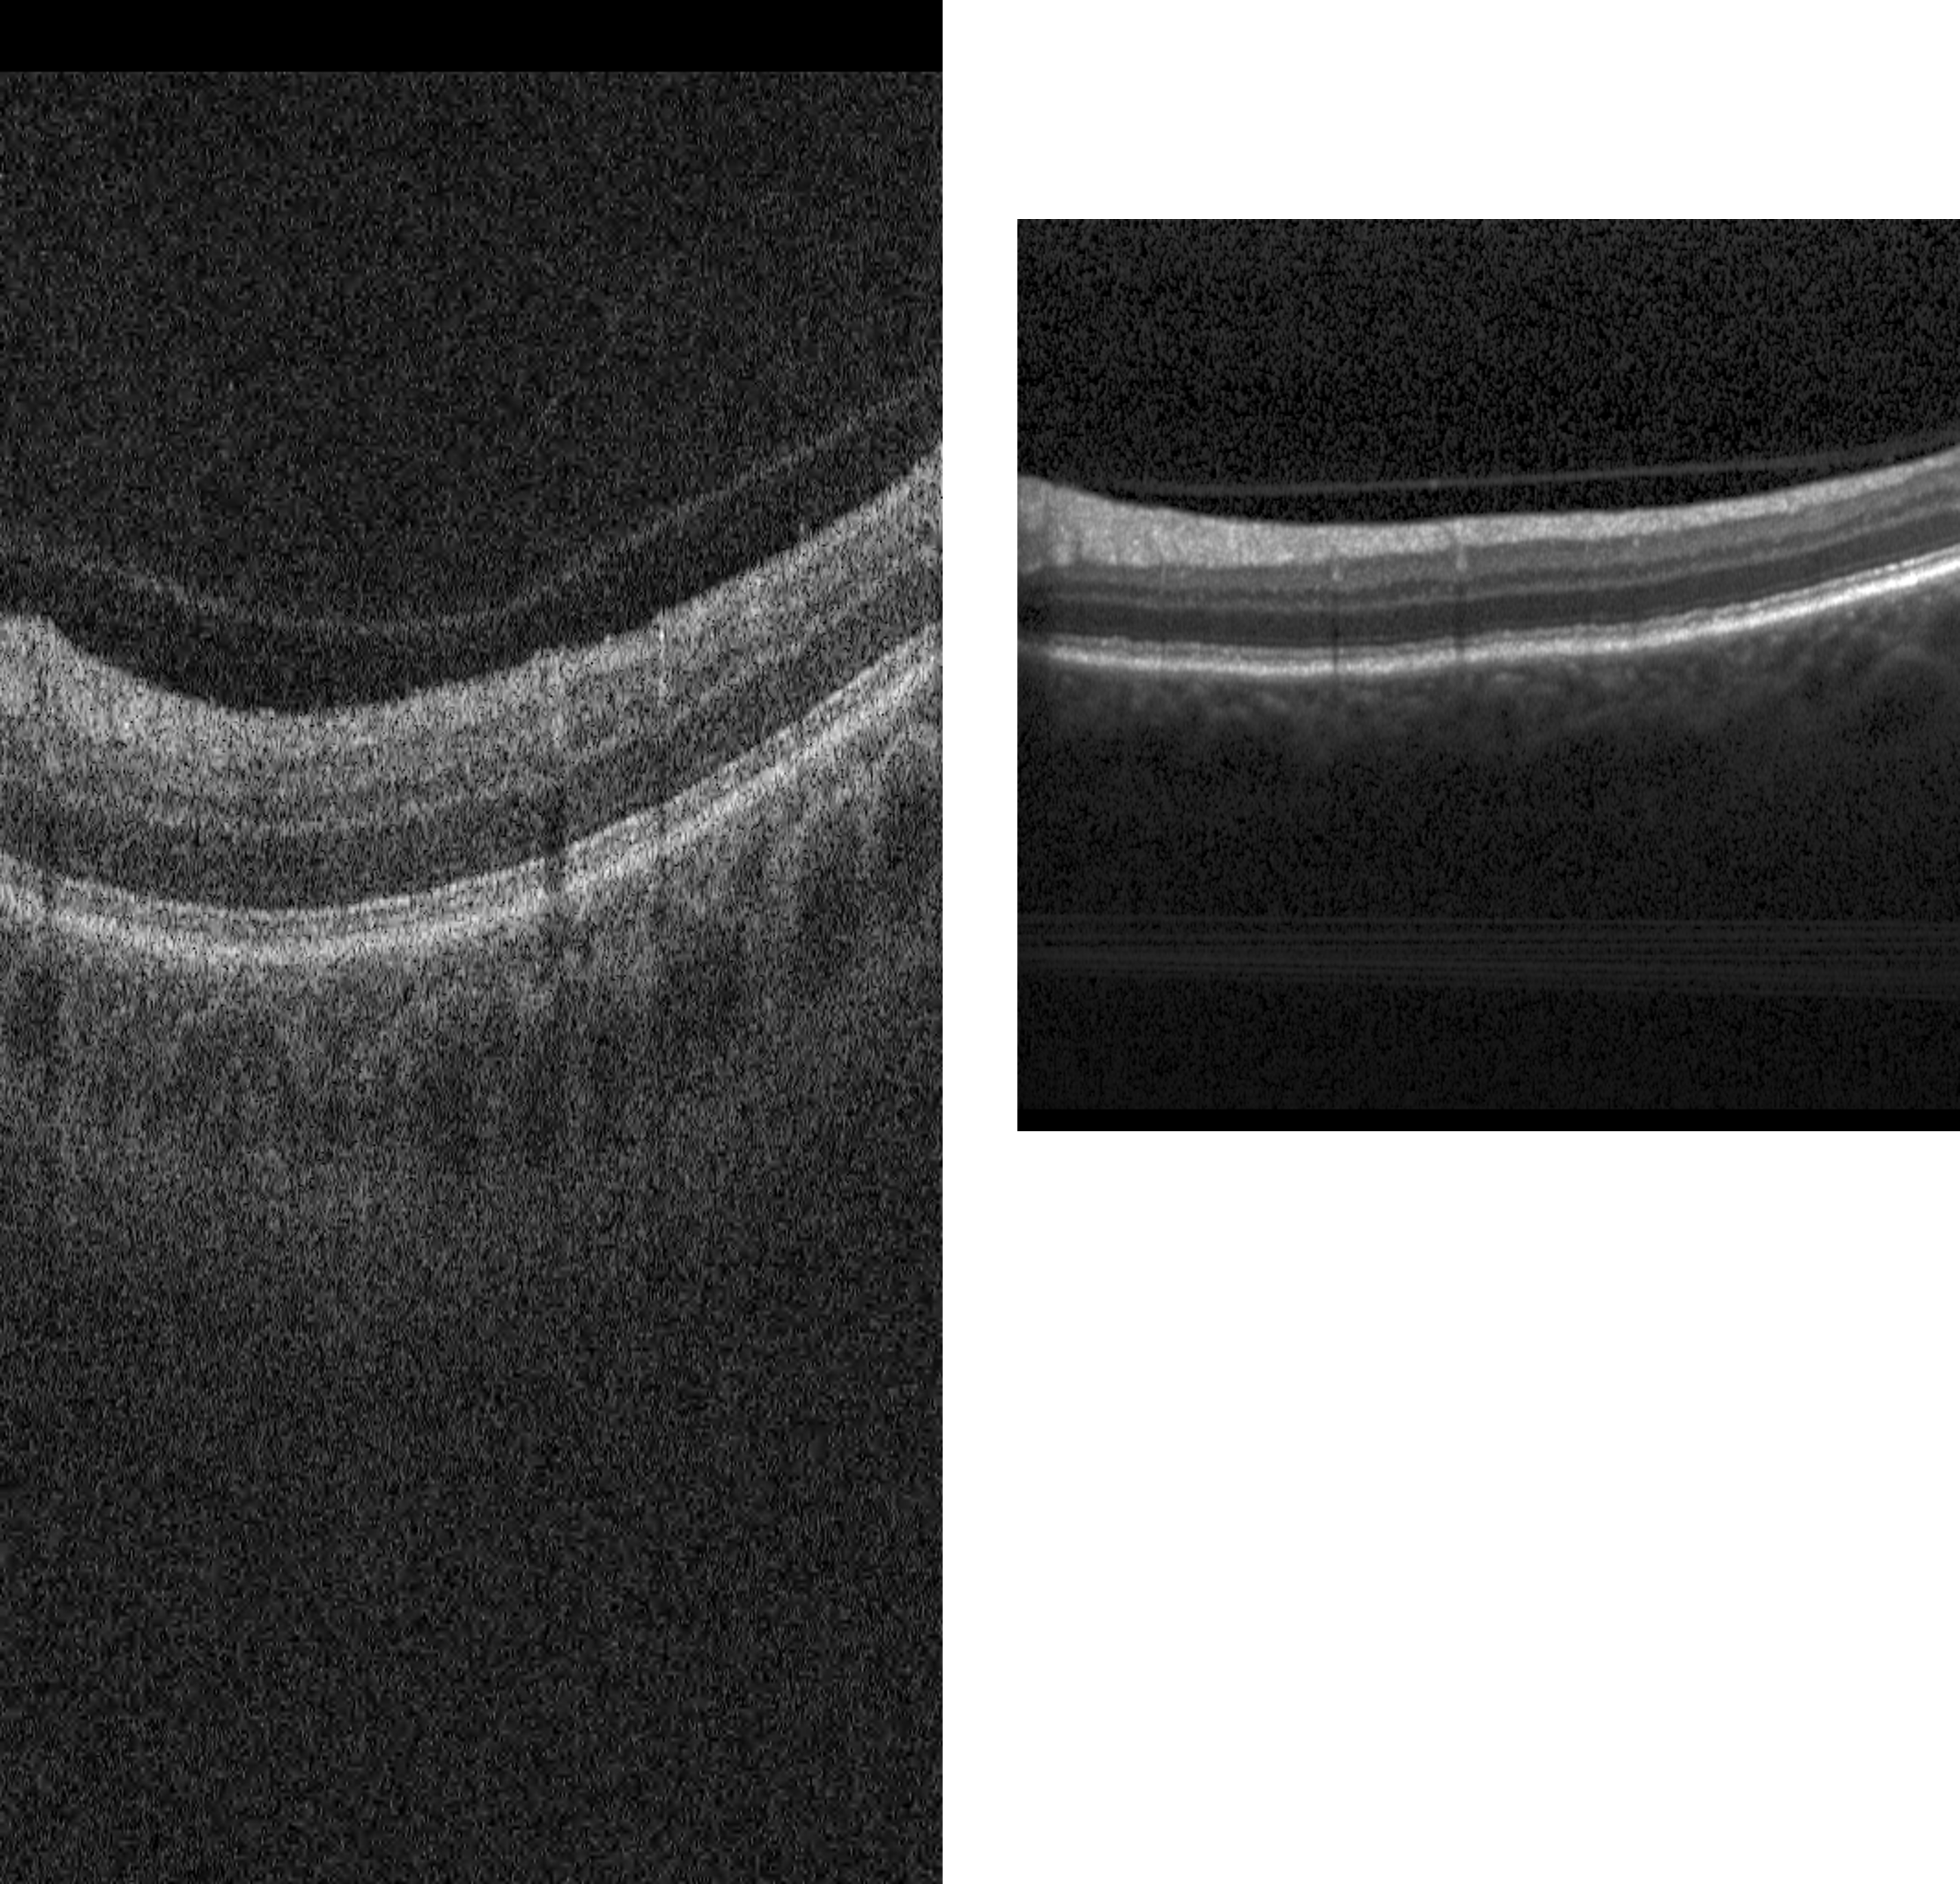
\includegraphics[width=0.4\linewidth]{figures/CirrusSpectralisRetinalLayerComparison.png}
	\caption{B-scan of the retinal layers in different patients, using Cirrus (left) and Spectralis (right) devices. In Cirrus, the retinal layers appear much larger than in Spectralis.}
	\label{fig:CirrusSpectralisRetinalLayerComparison}
\end{figure}

Then, vertical patches, of shape 496 $\times$ 128, were extracted from each B-scan. The number of patches extracted from each image was changed, experimenting with four (Figure \ref{fig:CirrusFourPatchExtraction}), seven (Figure \ref{fig:CirrusSevenPatchExtraction}) and thirteen (Figure \ref{fig:CirrusThirteenPatchExtraction}) patches. The advantage of extracting vertical patches is that each image contains both the complete retinal layer and the background. This does not happen in the previous experiments, where the patches are either too small to contain both background and the retinal layers (in Experiment 1.1) or the retinal layers are cropped during patch extraction (in Experiment 1.2, as seen in Figure \ref{fig:BigPatchExtraction}).

\begin{figure}[!ht]
	\centering
	\includegraphics[width=0.65\linewidth]{figures/CirrusFourPatchExtraction.png}
	\caption{Four vertical patches of shape 496 $\times$ 128 extracted from a Cirrus B-scan.}
	\label{fig:CirrusFourPatchExtraction}
\end{figure}

\begin{figure}[!ht]
	\centering
	\includegraphics[width=0.65\linewidth]{figures/CirrusSevenPatchExtraction.png}
	\caption{Seven vertical patches of shape 496 $\times$ 128 extracted from a Cirrus B-scan.}
	\label{fig:CirrusSevenPatchExtraction}
\end{figure}


\begin{figure}[!ht]
	\centering
	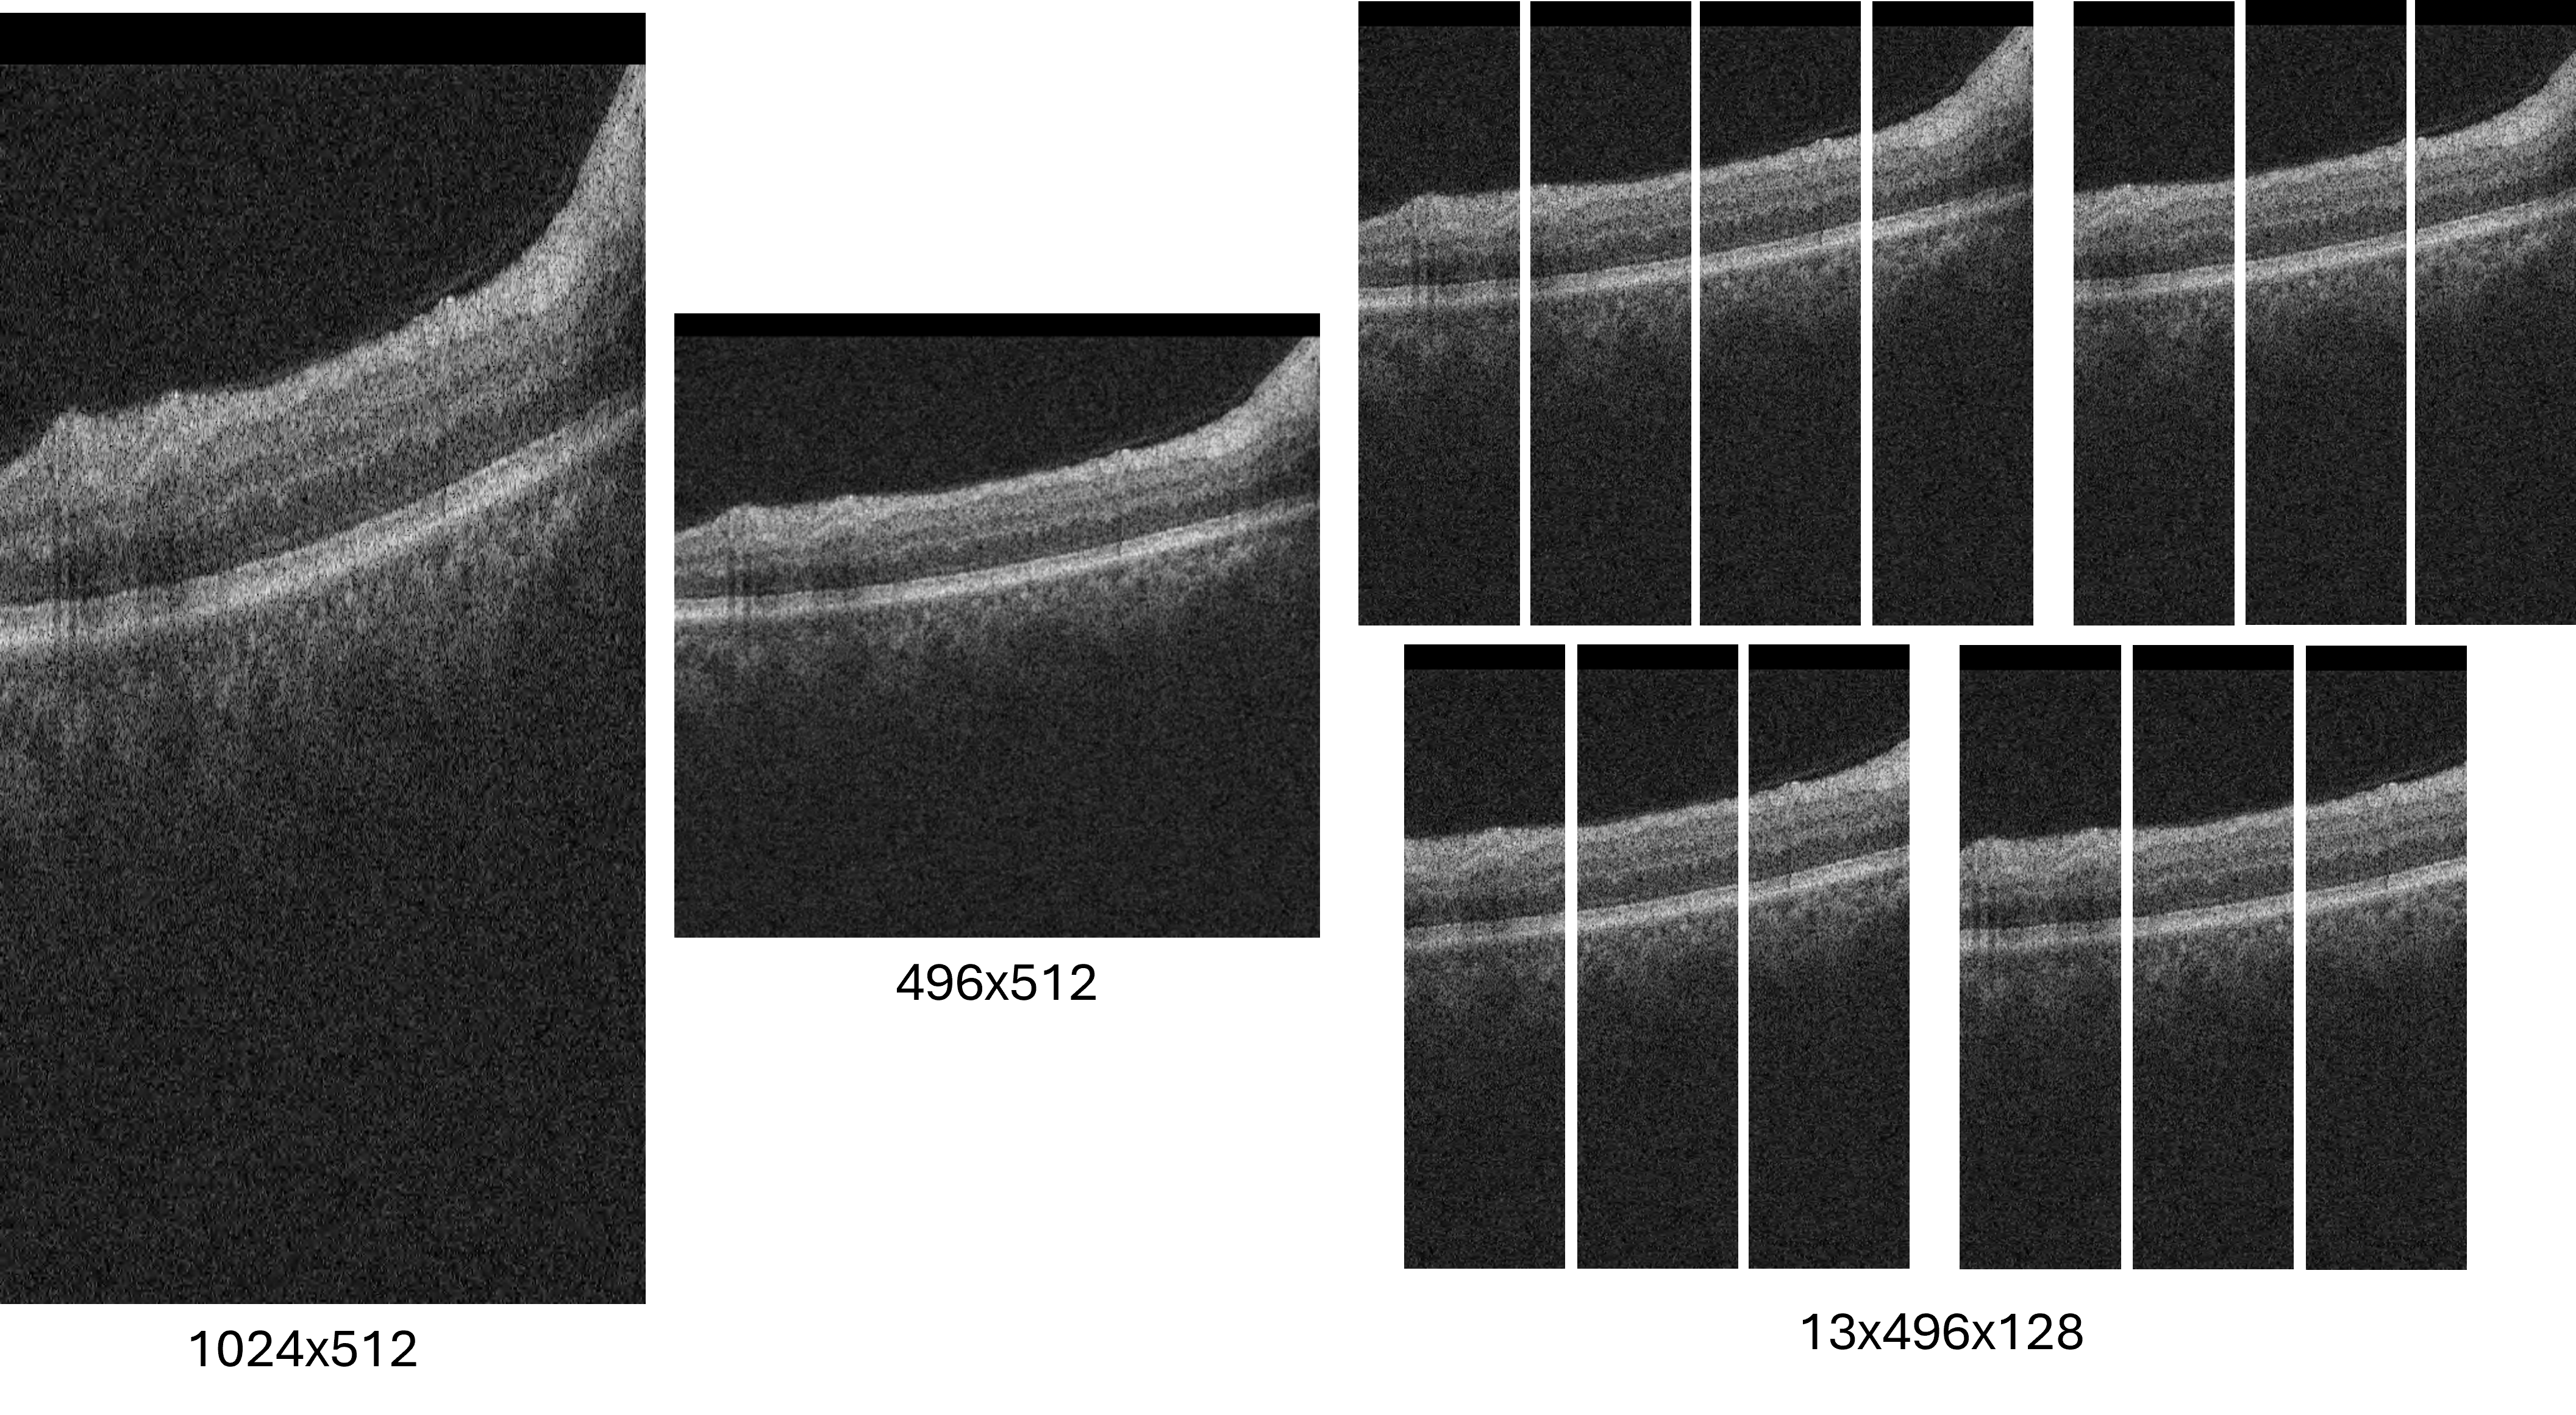
\includegraphics[width=0.75\linewidth]{figures/CirrusThirteenPatchExtraction.png}
	\caption{Thirteen vertical patches of shape 496 $\times$ 128 extracted from a Cirrus B-scan.}
	\label{fig:CirrusThirteenPatchExtraction}
\end{figure}

When using four vertical patches, the model was trained both for 100 and 200 epochs, maintaining a batch size of 32 and a maximum rotation of $10^{\circ}$, without early stopping. 
\par
Then, the model was trained using seven and thirteen patches for the best and worse performing folds when using four patches, while stopping early in case the validation loss did not progress 25 epochs after the minimum validation loss was encountered. This was used because the model progressed much faster when using seven and thirteen patches per B-scan, as it was trained in a much larger number of images per epoch. Henceforth, it also required more computational power, which further motivated the early stopping.
\par
Using seven vertical patches per image, which was the number of patches that performed best, three different rotations were experimented: no rotation, maximum rotation of $5^{\circ}$, and maximum rotation of $10^{\circ}$. These values were tested for a better understanding of how the rotation of the image affects the segmentation and the model's understanding of anatomic references. The models where rotation was applied were trained on a minimum of 100 epochs, after which a patience of 25 epochs was applied. Therefore, if after 100 epochs the model did not improve its validation loss for 25 consecutive epochs, then training would be interrupted. The models trained without rotation converged much faster and, for that reason, the minimum number of epochs used was 25, while still keeping the same patience. All models were trained for up to 200 epochs.
\par
Lastly, the model was trained using four patches and a maximum rotation of $5^{\circ}$, using the same early stopping criteria as in the last seven patches runs. This allowed for one last comparison between the two number of patches used in training, under the same conditions. The best model between those trained with four patches and those trained with seven patches was selected to infer on the reserved fold.

\subsubsection{Experiment 2}\label{Experiment2}
The second experiment also involved multi-class segmentation of the retinal fluids. Contrasting with the first experiment, where the segmentation was done using a U-Net, three U-Nets were used in this experiment, one for each fluid. Each U-Net model focused only on the segmentation of one fluid, with one model for IRF, one for SRF, and one for PED.
\par
One of the main problems with multi-class segmentation performed by binary models is the merging of the multiple masks. In this context, multiple fluid classes can be predicted for the same voxel, while only one of those can be correct. In this experiment, two alternatives were explored: order of priority, where the merging of the fluid masks follows a predefined hierarchy that determines which fluid takes precedence, and highest probability, where the assigned class is the one that was predicted with highest probability by its model.
\par
Two different losses were used to regulate the model. Initially, the same loss as the one used in \ref{Experiment1} Experiment 1, with only two classes (background and the fluid that would be segmented), and then, the weighted cross-entropy, using weights that balance the larger quantity of background voxels. This last loss is described in Equation \ref{eq:SegmentationCE}, with $N=2$.
\par
When using the loss from \ref{Experiment1} Experiment 1, each model was trained on two different splits: the split used in the multi-class segmentation experiments and a split created specifically for the segmentation of the fluid that was being segmented. 
\par
The balanced cross-entropy loss was tested on the best performing folds of the multi-class and IRF splits, for the segmentation of IRF, in the same conditions. However, since the results were much worse than those obtained with the initial loss, no more folds or fluids were considered.
\par
All the models were trained with seven vertical patches extracted from each B-scan, on a minimum of 100 epochs, after which a patience of 25 epochs was applied, like what was done in the last runs of \ref{Experiment1} Experiment 1. Similarly, the random transformations applied to the images consisted of horizontal flipping and a maximum rotation of $5^{\circ}$.

\subsection{Intermediate Slice Synthesis}
The objective of the subsequent experiments is to improve the resolution between slices, thus approximating the estimated fluid volume to the true value.
\par
The intermediate slices were generated using the RETOUCH dataset as training and validation data. In this experiment, subvolumes that consist of overlapping triplets of consecutive slices, sampled with a step size of 1, were used, extracted as shown in Figure \ref{fig:FrameInterpolationFramework}. The first and the last slice of these triplets were used for the generation of the middle slice. Consequently, it is possible to evaluate the generated slice in comparison to the original one, as done in other examples of the literature. For each volume, the number of potential subsets is then determined to be $n-2$, where $n$ represents the number of slices within the same volume.

\begin{figure}[!ht]
	\centering
	\includegraphics[width=1.0\linewidth]{figures/FrameInterpolationFramework.png}
	\caption{Scheme explaining the input data of the generative models. Each frame refers to B-scan from an OCT volume. Extracted from \textcite{Tran2020}.}
	\label{fig:FrameInterpolationFramework}
\end{figure}

The generation of slices can be evaluated in specific metrics, as well as through qualitative assessment. To assess the efficacy of the generation model, the model utilized for fluid segmentation could be used for the estimation of the fluid's area in the generated image and to compare the resulting mask with the original image's mask. This comparison can be conducted using the Dice coefficient \parencite{Lopez2023} (see Equation \ref{eq:DiceCoefficientPixels}). However, this metric is insufficient for evaluating the generation performance, as it requires comparisons that encompass the entire slice and not just the fluid region. Examples of such metrics include the mean absolute error (MAE) \parencite{Lopez2023, Wu2022, Zhang2022}, the peak signal-to-noise ratio (PSNR) \parencite{Xia2021, YChen2018, Sanchez2018, Fang2022, Nimitha2024, Kudo2019, You2020, Zhang2024, Zhang2022}, and the structural similarity index measure (SSIM) \parencite{YChen2018, Sanchez2018, Fang2022, Nimitha2024, Kudo2019, You2020, Zhang2024, Zhang2022}.
\par
The MAE and mean squared error (MSE) quantify the errors between the original image and the generated image. For every pixel, the difference between the value in the original image and the generated image is calculated. In MAE, the absolute value of this difference is calculated, and then the mean of all pixels in the image is computed. Meanwhile, in MSE, the difference is squared before computing the mean. In Equation \ref{eq:MAEEquation} and Equation \ref{eq:MSEEquation}, MAE and MSE are described, respectively, where $x_{i}$ is the intensity of the pixel of index $i$ in the predicted image, while $y_{i}$ is the intensity of the pixel with index $i$ in the original image, and $N$ is the number of pixels in the image \parencite{Sara2019, Rajkumar2016}.

\begin{equation}
	\text{MAE} = \frac{1}{N} \sum_{i=1}^{N} |x_i - y_i|
	\label{eq:MAEEquation}
\end{equation}

\begin{equation}
	\text{MSE} = \frac{1}{N} \sum_{i=1}^{N} \left( x_i - y_i \right)^{2}
	\label{eq:MSEEquation}
\end{equation}

PSNR is a metric used to calculate the ratio between the maximum signal power (which corresponds to the maximum value of a pixel in the image) and the power of the distorting noise, which affects the quality of its representation. Therefore, the PSNR, described in Equation \ref{eq:PSNREquation}, is inversely proportional to the mean squared error. PSNR can also be understood as the representation of absolute error in dB \parencite{Sara2019}. It is important to note that in OCT the signal-to-noise ratio is low, due to the speckle present in the images. Therefore, a smaller PSNR is also expected, when compared with other imaging techniques that do not present as much speckle \parencite{Bogunovic2019a}.

\begin{equation}
	\text{PSNR} = 10 \cdot \log_{10} \left( \frac{L^2}{\text{MSE}} \right)
	\label{eq:PSNREquation}
\end{equation}

While the previous metrics focus on the differences between two images at a pixel level, the SSIM is based on the perception of the image. This metric considers the change of perception in structural information, estimating the perceived quality of images and videos. SSIM measures the similarity between the original image and the generated. The SSIM is calculated as shown in Equation \ref{eq:SSIMEquation}, where $x$ and $y$ represent the generated and the original images, respectively, so that $\mu_{x}$ and $\mu_{y}$ are their local means, $\sigma_{x}$ and $\sigma_{y}$ are their standard deviations, while $C_{1}$ and $C_{2}$ are small constants that stabilize the division. The contrast sensitivity (CS) between the images $x$ and $y$ is represented by $CS(x,y)$ \parencite{Sara2019}.

\begin{equation}
	\text{SSIM}(x, y) = \left( \frac{2\mu_x \mu_y + C_1}{\mu_x^2 + \mu_y^2 + C_1} \right) \cdot \left( \frac{2\sigma_{xy} + C_2}{\sigma_x^2 + \sigma_y^2 + C_2} \right) = \left( \frac{2\mu_x \mu_y + C_1}{\mu_x^2 + \mu_y^2 + C_1} \right) \cdot CS(x, y)
	\label{eq:SSIMEquation} 
\end{equation}

Since the best performing models in segmentation resized the images to 496 $\times$ 512, the images were generated to match those dimensions. Therefore, regardless of the device utilized to obtain the OCT volume, all its B-scans were resized to 496 $\times$ 512 for both experiments of image generation.

\subsubsection{Experiment 3}
In the first experiment focused on intermediate slice synthesis, a GAN was used. The underlying principle of a GAN, originally proposed by \textcite{Goodfellow2014}, is based on a competitive game between two networks. The generator network starts with the first and last slice of a subvolume, which is composed of three consecutive B-scans from an OCT scan, and aims to generate the intermediate slice. In contrast, the discriminator network is trained to distinguish between the generated and real slices. When the discriminator correctly labels generated slices as fake, the generator is penalized, motivating it to fool the discriminator and consequently improving its generation, resulting in outputs more similar to the real inputs. However, the discriminator network loss also penalizes misclassifications, dependent on the probability of the prediction. As a result, as the generator improves, so does the discriminator \parencite{Goodfellow2020}. The overall framework for GANs is illustrated in Figure \ref{fig:GANFramework}.

\begin{figure}[!ht]
	\centering
	\includegraphics[width=0.7\linewidth]{figures/GANFramework}
	\caption{Example of a GAN framework, where $\mathcal{D}$ is the discriminator and $\mathcal{G}$ is the generator \cite{Creswell2018}.}
	\label{fig:GANFramework}
\end{figure}

The GAN implemented by \textcite{Tran2020} was used to generate the intermediate slices of the OCT volumes. This framework is used in the interpolation of intermediate slices in video and is trained in patches of 64 $\times$ 64.
\par
In the original implementation, one patch is randomly extracted from the triplet of images and used in training. Due to the much smaller quantity of data available in OCT, all the possible disjoint 64 $\times$ 64 patches were extracted from each B-scan. The extraction was done from top to bottom and in the last row of slices, the image was padded until it had 64 pixels. An example of the patches extracted from a Cirrus B-scan can be seen in Figure \ref{fig:CirrusSixtyFourPatchExtraction}. By methodically extracting the patches, triplets are easily created by accessing patches of the same index in the three consecutive images.

\begin{figure}[!ht]
	\centering
	\includegraphics[width=0.7\linewidth]{figures/CirrusSixtyFourPatchExtraction.png}
	\caption{Patches with shape 64 $\times$ 64 extracted from a Cirrus B-scan which was resized to 496 $\times$ 512.}
	\label{fig:CirrusSixtyFourPatchExtraction}
\end{figure}

The generator of the GAN is composed of contracting and expanding path. In the contracting path, convolutions are applied to the images and feature maps, followed by batch normalization, and a leaky ReLU activation function. After the images are downsampled to 512 $\times$ 8 $\times$ 8, reaching the bottleneck, the expanding path begins, where deconvolutions are applied, followed by batch normalization, and a leaky ReLU. Finally, after the last deconvolution, the hyperbolic tangent function is used as the final activation function, resulting in an output of size 64 $\times$ 64, in range -1 to 1. An illustrative scheme of the generator can be seen in Figure \ref{fig:GeneratorArchitecture}.

\begin{figure}
	\centering
	\includegraphics[width=1.0\linewidth]{figures/GeneratorArchitecture}
	\caption{Architecture of the generator used in the GAN. It has a contracting and an expanding path, making it a U-Net like network \parencite{Tran2020}.}
	\label{fig:GeneratorArchitecture}
\end{figure}


To match the needs of our application, some changes had to be made in the generator regarding the input shape. As shown in Figure \ref{fig:GeneratorArchitecture}, the input has six channels, one red, one green, and one blue (RGB) for each input patch. Similarly, the output has three channels, for the generated middle patch. In our application, each patch in the input only had one channel, since the OCT B-scans are images in gray scale, instead of RGB, as in the original implementation. Therefore, the output only had one channel. 
\par
The final activation function, the hyperbolic tangent, outputs values between -1 and 1. Since the output images were compared to images in range 0 to 1, the final activation function was changed to the sigmoid. This function converts the values output from the last convolution to the range of 0 to 1, where it can be compared to the GT images.
\par
The GAN's discriminator receives as input a patch of shape 64 $\times$ 64, and outputs a probability of the input patch being real. The discriminator is composed of five consecutive convolutions. The first convolution is followed by a leaky ReLU activation function. The second, third, and fourth convolutions are followed by a batch normalization and a leaky ReLU activation function. After the last convolution, the sigmoid is applied and converts the final output to a value between 0 and 1 that represents the probability of the image being real. In Table \ref{tab:GeneratorDiscriminatorArchitecture}, the layers that compose the discriminator and the generator are explained, including the shape of the outputs.

\begin{table*}[!ht]
	\setlength{\tabcolsep}{6pt}
	\renewcommand{\arraystretch}{1.3}
	\caption{Layers that compose the generator and the discriminator. Each convolution is represented by Conv2d(K, OC, S), where K is the kernel size, OC is the number of output channels, and S is the stride. The same notation is used in deconvolutions, represented by TransposedConv2d. The output size is shown following C $\times$ H $\times$ W notation, where C is the number of channels, H is the height, and W is the width. The inputs have shape $1 \times 64 \times 64$. Adapted from \textcite{Tran2020}.}
	\centering
	\resizebox{\textwidth}{!}{\begin{tabular}{c c c}
		\hline
		\hline
		\multicolumn{3}{c}{\textbf{Generator}} \\
		\hline
		\textbf{Layers} & \textbf{Details} & \textbf{Output Size (C $\times$ H $\times$ W)} \\
		\hline
		\textbf{1} & Conv2d(3, 128, 1), BatchNorm2d, LeakyReLU & 128 $\times$ 64 $\times$ 64 \\
		\textbf{2} & Conv2d(4, 128, 2), BatchNorm2d, LeakyReLU & 128 $\times$ 32 $\times$ 32 \\
		\textbf{3} & Conv2d(4, 256, 2), BatchNorm2d, LeakyReLU & 256 $\times$ 16 $\times$ 16 \\
		\textbf{4} & Conv2d(4, 512, 2), BatchNorm2d, LeakyReLU & 512 $\times$ 8 $\times$ 8 \\
		\textbf{5} & TransposedConv2d(4, 256, 2), BatchNorm2d, LeakyReLU & 256 $\times$ 16 $\times$ 16 \\
		\textbf{6} & TransposedConv2d(4, 128, 2), BatchNorm2d, LeakyReLU & 128 $\times$ 32 $\times$ 32 \\
		\textbf{7} & TransposedConv2d(4, 64, 2), BatchNorm2d, LeakyReLU & 64 $\times$ 64 $\times$ 64 \\
		\textbf{8} & TransposedConv2d(1, 1, 1), Sigmoid & 1 $\times$ 64 $\times$ 64 \\
		\hline
		\hline
		\multicolumn{3}{c}{\textbf{Discriminator}} \\
		\hline
		\textbf{Layers} & \textbf{Details} & \textbf{Output Size (C $\times$ H $\times$ W)} \\
		\hline
		\textbf{1} & Conv2d(4, 64, 2), LeakyReLU & 64 $\times$ 32 $\times$ 32 \\
		\textbf{2} & Conv2d(4, 128, 2), BatchNorm2d, LeakyReLU & 128 $\times$ 16 $\times$ 16 \\
		\textbf{3} & Conv2d(4, 256, 2), BatchNorm2d, LeakyReLU & 256 $\times$ 8 $\times$ 8 \\
		\textbf{4} & Conv2d(4, 512, 2), BatchNorm2d, LeakyReLU & 512 $\times$ 4 $\times$ 4 \\
		\textbf{5} & Conv2d(4, 1, 1), Sigmoid & 1 $\times$ 1 $\times$ 1 \\
		\hline
		\hline
	\end{tabular}}
	\label{tab:GeneratorDiscriminatorArchitecture}
\end{table*}

In the training of a GAN, both the generator and the discriminator are being trained sequentially and independently. First, the generator, which receives the previous and following patch of the input triplet, attempts to generate the intermediate patch. The generated image is then compared to the original image, using the generator loss, which is then used in the updating of the generator weights. The generator loss is composed of four components: the adversarial, the MAE, the multi-scale SSIM (MS-SSIM), and the gradient difference loss (GDL). The overall loss function is described in Equation \ref{eq:GeneratorLoss}, where $\lambda_{\text{adv}}=0.05$, $\lambda_{\text{MAE}}=1.0$, $\lambda_{\text{MS-SSIM}}=6.0$, and $\lambda_{\text{GDL}}=1.0$, representing the weights of each loss component.

\begin{equation}
	\mathcal{L}_{\text{Gen}} = \lambda_{\text{adv}} \times \mathcal{L}_{\text{adv}} + \lambda_{\text{MAE}} \times \mathcal{L}_{\text{MAE}} + \lambda_{\text{MS-SSIM}} \times \mathcal{L}_{\text{MS-SSIM}} + \lambda_{\text{GDL}} \times \mathcal{L}_{\text{GDL}}
	\label{eq:GeneratorLoss}
\end{equation}

The adversarial loss is used in the evaluation of how good the output from the generator fools the discriminator. This evaluation is done using the binary cross-entropy (BCE). To calculate this, the generated image is input into the discriminator, which then outputs the probability of being real. Afterwards, the BCE is calculated for the predicted probability and 1, the label of a real image. The better the generator fools the discriminator, the closer the output of the discriminator is to one, and, therefore, the closer the adversarial loss is to 0. The adversarial loss is explained in Equation \ref{eq:AdversarialLoss}, where $\mathcal{D}$ is the discriminator, $x$ is the generated image, and $y$ is the label that indicates that the image is real. It is important to note that in the generator training, the images that are input to the discriminator are detached, not contributing to the updating of the discriminator weights in this step.

\begin{equation}
	\mathcal{L}_{\text{adv}} (\mathcal{D}(x), y) = \mathcal{L}_{\text{BCE}} (\mathcal{D}(x), y) = - \left[ y \text{log}(\mathcal{D}(x)) + (1 - y)\text{log}(1 - \mathcal{D}(x)) \right]
	\label{eq:AdversarialLoss}
\end{equation}

The MAE loss, also referred to as $L_{1}$ loss, performs a pixel-by-pixel comparison between the generated image, $x$, and the real image, $y$, as described in Equation \ref{eq:MAEEquation}, where $i$ is the index of a pixel. While this loss gives an insight of how similar the images are, on average, this loss can be deceiving, since the model can blur the output to attain better MAE values. For this reason, this loss must be combined with other reconstructive losses, such as the MS-SSIM and the GDL.
\par
The MS-SSIM loss seeks to preserve the structural similarity, at different scales, between the real and the generated image, facilitating a smoother output. This loss, originally suggested by \textcite{Wang2003}, is described in Equation \ref{eq:MSSSIMLoss}, while the MS-SSIM used in this implementation is explained in Equation \ref{eq:MSSSIM}, using the concepts of SSIM and CS explained in Equation \ref{eq:SSIMEquation}. This version of the MS-SSIM is faster than the original implementation \parencite{Wang2003}, while using the same array of weights $\beta$ and number of levels $M$, which is set to 5. Therefore, the MS-SSIM corresponds to the product of the contrast sensitivity in the image for first four levels and the SSIM of the image in the last level, all raised to the power of the respective level's weights.

\begin{equation}
	\mathcal{L}_{\text{MS-SSIM}} (x, y) = 1 - \text{MS-SSIM}(x, y)
	\label{eq:MSSSIMLoss}
\end{equation}

\begin{equation}
	\text{MS-SSIM}(x, y) = \prod_{j=1}^{M-1} \left[ \text{CS}_j(x, y) \right]^{\beta_j} \cdot \left[ \text{SSIM}_M(x, y) \right]^{\beta_M}
	\label{eq:MSSSIM}
\end{equation}

The last component of the loss is the GDL, proposed originally by \textcite{Mathieu2016}. This component is used to reduce the motion blur in the generated images, a problem in video datasets. In this loss, the relative difference of neighboring pixels between the generated and true images is considered, as shown in Equation \ref{eq:GDLLoss}. In this equation, $i$ and $j$ are the index of row and column, respectively, that identify a pixel of the image, with $\alpha$ set to 2.

\begin{equation}
	\mathcal{L}_{\text{GDL}}(x, y) = \sum_{i,j} \left( \left|\,|x_{i,j} - x_{i-1,j}| - |y_{i,j} - y_{i-1,j}|\,\right|^{\alpha} + \left|\,|x_{i,j} - x_{i,j-1}| - |y_{i,j} - y_{i,j-1}|\,\right|^{\alpha} \right)
	\label{eq:GDLLoss}
\end{equation}

After the images are generated and evaluated using the previously defined generator loss, two images are input, subsequently, to the discriminator, with one of them being fake while the other is real. The discriminator outputs the probability of each image being real and its result is compared to the true label of each image using the BCE. The BCE is calculated for the probabilities predicted by the discriminator and the image's respective label as described in Equation \ref{eq:AdversarialLoss}. This is done for the fake image and for the real image. The mean between the BCE calculated for the fake image and the BCE computed for the real image is the discriminator loss.
\par
The GAN was trained in 250 epochs, using a batch size of 32 and $2 \times 10^{-4}$ as the learning rate. The selected optimizer was Adam, with $\beta_{1}=0.5$ and $\beta_{2}=0.999$.

\subsubsection{Experiment 4}
As in the previous experiment, the intermediate slice was generated using the first and last slices of a subvolume that consists of three consecutive B-scans from an OCT scan. However, in this experiment, inspired by the work of \textcite{Nishimoto2024}, the intermediate slice was generated using a U-Net. While the U-Net is more commonly applied in segmentation, as seen in the reviewed literature, \textcite{Nishimoto2024} apply it to generate the intermediate slices of a subvolume. The U-Net receives the edge slices as input and forces the output of the intermediate ones. In the paper \parencite{Nishimoto2024}, this was tested for three, four, and five slices. However, in this experiment it was utilized to generate a single intermediate slice.
\par
In this experiment, the whole image is input to the network and for that reason the batch size was set to 8. The optimizer utilized was Adam with a learning rate of $2 \times 10^{-4}$ and the model was trained for 200 epochs.

\subsection{Fluid Volume Estimation}
The estimation of fluid volume was done using the optimal segmentation and intermediate slice generation models. The GAN was used in the generation of the intermediate slices in the OCT volumes, while the best performing multi-class segmentation U-Net model inferred the segmentation masks to both the unaltered volumes and the volumes with generated slices. 
\par
The OCT scans used in the fluid volume estimation experiments were the ones from the \hbox{RETOUCH} dataset that composed the reserved fold in the segmentation and generation experiments and the ones from the private dataset obtained in Hospital São João. These volumes were selected because no model was trained or validated on them, allowing an insight of both models generalization on unseen data and how the increase in resolution affects the total fluid volume.
\par
The area of each fluid in each OCT scan was estimated considering the resolution of each OCT scan, which varies according to the device utilized to obtain the OCT volume. Afterwards, the area is multiplied by the axial distance (half the axial distance to the previous slice plus half the axial distance to the following slice) to obtain the volume of fluid per slice. In the first and last slice of an OCT volume, the area is multiplied by half of the axial distance (half the axial distance to the neighboring slice). The total volume of fluid in an OCT scan can be estimated by summing the fluid volumes of all individual B-scans. This allows the volume estimation of IRF, SRF, and PED, as well as the overall fluid volume in the OCT scan.
\par
The total volume of fluid from class $c$ in a slice of index $s$ is defined in Equation \ref{eq:FluidEstimationSlice}. The slice belongs to an OCT volume obtained using device $D$ and its total number of B-scans is defined as $S$. In this equation, $H_{D}$ and $W_{D}$ are the height and width of a voxel, respectively, obtained with device $D$, while $d_{D,s,s+1}$ is the axial distance between the slice of index $s$ and the slice of index $s+1$, a value that depends on the device $D$ characteristics. The variable $l_{i}$ is the label attributed to the voxel of index $i$. Like the variable $c$, $l$ can be one of the following classes: $\{0,1,2,3\}$, which respectively correspond to background, IRF, SRF, and PED. Meanwhile, the total volume of fluid from a class $c$ in an OCT scan obtained with device $D$ is described by Equation \ref{eq:FluidEstimationVolume}, and consists of the sum of the fluid's volume obtained in each B-scan that compose the OCT.

\begin{equation}
	\begin{aligned}
		f_{c,s,D} &= \sum_{i} \left( v_{i,s,D} \times y_{i,c} \right) \quad \text{where: }\\
		v_{i,s,D} &=
		\begin{cases}
			0.5 \times H_{D} \times W_{D} \times d_{D,s,s+1} & \text{if $s=0$}\\
			0.5 \times H_{D} \times W_{D} \times d_{D,s,s-1} & \text{if $s=S$}\\
			0.5 \times H_{D} \times W_{D} \times d_{D,s,s-1} + 0.5 \times H_{D} \times W_{D} \times d_{D,s,s+1} & 
			\text{otherwise}\\
		\end{cases}\\
		y_{i,c} &=
		\begin{cases}
			1 &\text{if } l_{i} = c\\
			0 &\text{if } l_{i} \neq c\\
		\end{cases} 
		\label{eq:FluidEstimationSlice}
	\end{aligned}
\end{equation}

\begin{equation}
	F_{c,D} = \sum_{s}^{S} f_{c,s,D}
	\label{eq:FluidEstimationVolume}
\end{equation}

The fluid volumes resulting from both experiments were compared. Since there is no true value for the fluid quantity in the OCT scans, the results were compared with each other. Therefore, the results would be deemed satisfying in case they do not vary more than an order of magnitude between each other. In case a significant difference was observed, the generated images and their respective masks were analyzed, in order to understand what is causing the observed difference between experiments.

\subsubsection{Experiment 5}
In this experiment, the fluid volumes were calculated for the OCT scans without the generated slices. The best segmentation model was utilized to segment the fluid in three classes and the volume was estimated for each class as described. The results from this experiment allow the comparison with the values obtained in the following experiment, where slice generation was used.

\subsubsection{Experiment 6}
This experiment consisted of the fluid volume estimation in OCT scans with generated images. The model used in segmentation was the same as in the previous experiment, which predicted the fluid masks for all the slices. From the predicted fluid masks, the fluid volume was estimated and compared with those obtained in the previous experiment. 